\chapter{Data Summary}
\label{app:data}
\section*{Kraka}
\begin{table}
\centering
\caption{Kraka Survey Parameters}
\label{kraka-label}
\begin{tabular}{|l|ccccc|}
\hline
\rowcolor[HTML]{C0C0C0}Survey & \cellcolor[HTML]{C0C0C0}KRAKA90 & \cellcolor[HTML]{C0C0C0}KRAKA00 & \cellcolor[HTML]{C0C0C0}ES02 & \cellcolor[HTML]{C0C0C0}DUC05 & \cellcolor[HTML]{C0C0C0}DUC12  \\ \hline
Direction [$^o$] & 90 & 305 & 90 & 90 & 90 \\ \hline
Inline Spacing [m] &  & 12.5 & 25 & 6.25 & 6.25 \\ \hline
Crossline Spacing [m] &  & 12.5 & 12.5 & 25 & 25 \\ \hline
Undershoot &  & No &  & Yes & Yes \\ \hline
\rowcolor[HTML]{C0C0C0} Energy Source & \multicolumn{5}{l|}{\cellcolor[HTML]{C0C0C0}}  \\ \hline
Number of Arrays  & 1 & 2 & 2 & 2 & 2 \\ \hline
Array Volume [cu.ins.] &  3360  &  & 3090 & 3147 & 3450 \\ \hline
Source Depth [m] & 5 &  & 6 & 5 & 5 \\ \hline
\rowcolor[HTML]{C0C0C0}Streamer Parameters & \multicolumn{5}{l|}{\cellcolor[HTML]{C0C0C0}} \\ \hline
Number of Streamers & 4 & 6 & 8 & 8 & 8 \\ \hline
Separation [m] & 30 &  &  & 100 & 100 \\ \hline
Length [m] & 288 &  & 5100 & 6000 & 4040 \\ \hline
Number of Groups & 24 & 408 & 408 & 478 & 324 \\ \hline
Group Interval [m] & 12.5 &  & 12.5 & 12.5 & 12.5 \\ \hline
Depth [m] & 8 &  & 7 & 7 & 7 \\ \hline
Near Offset [m] & 80 &  &  & 287 & 102 \\ \hline
\rowcolor[HTML]{C0C0C0}Recording System& \multicolumn{5}{l|}{\cellcolor[HTML]{C0C0C0}} \\ \hline
Low Filter Cut-Off [Hz] & 3 & 4 & 3 & 3 & 3 \\ \hline
Low Filter Flank [dB/Oct] & 6 & 18 & 6 & 18 & 6 \\ \hline
\end{tabular}
\end{table}
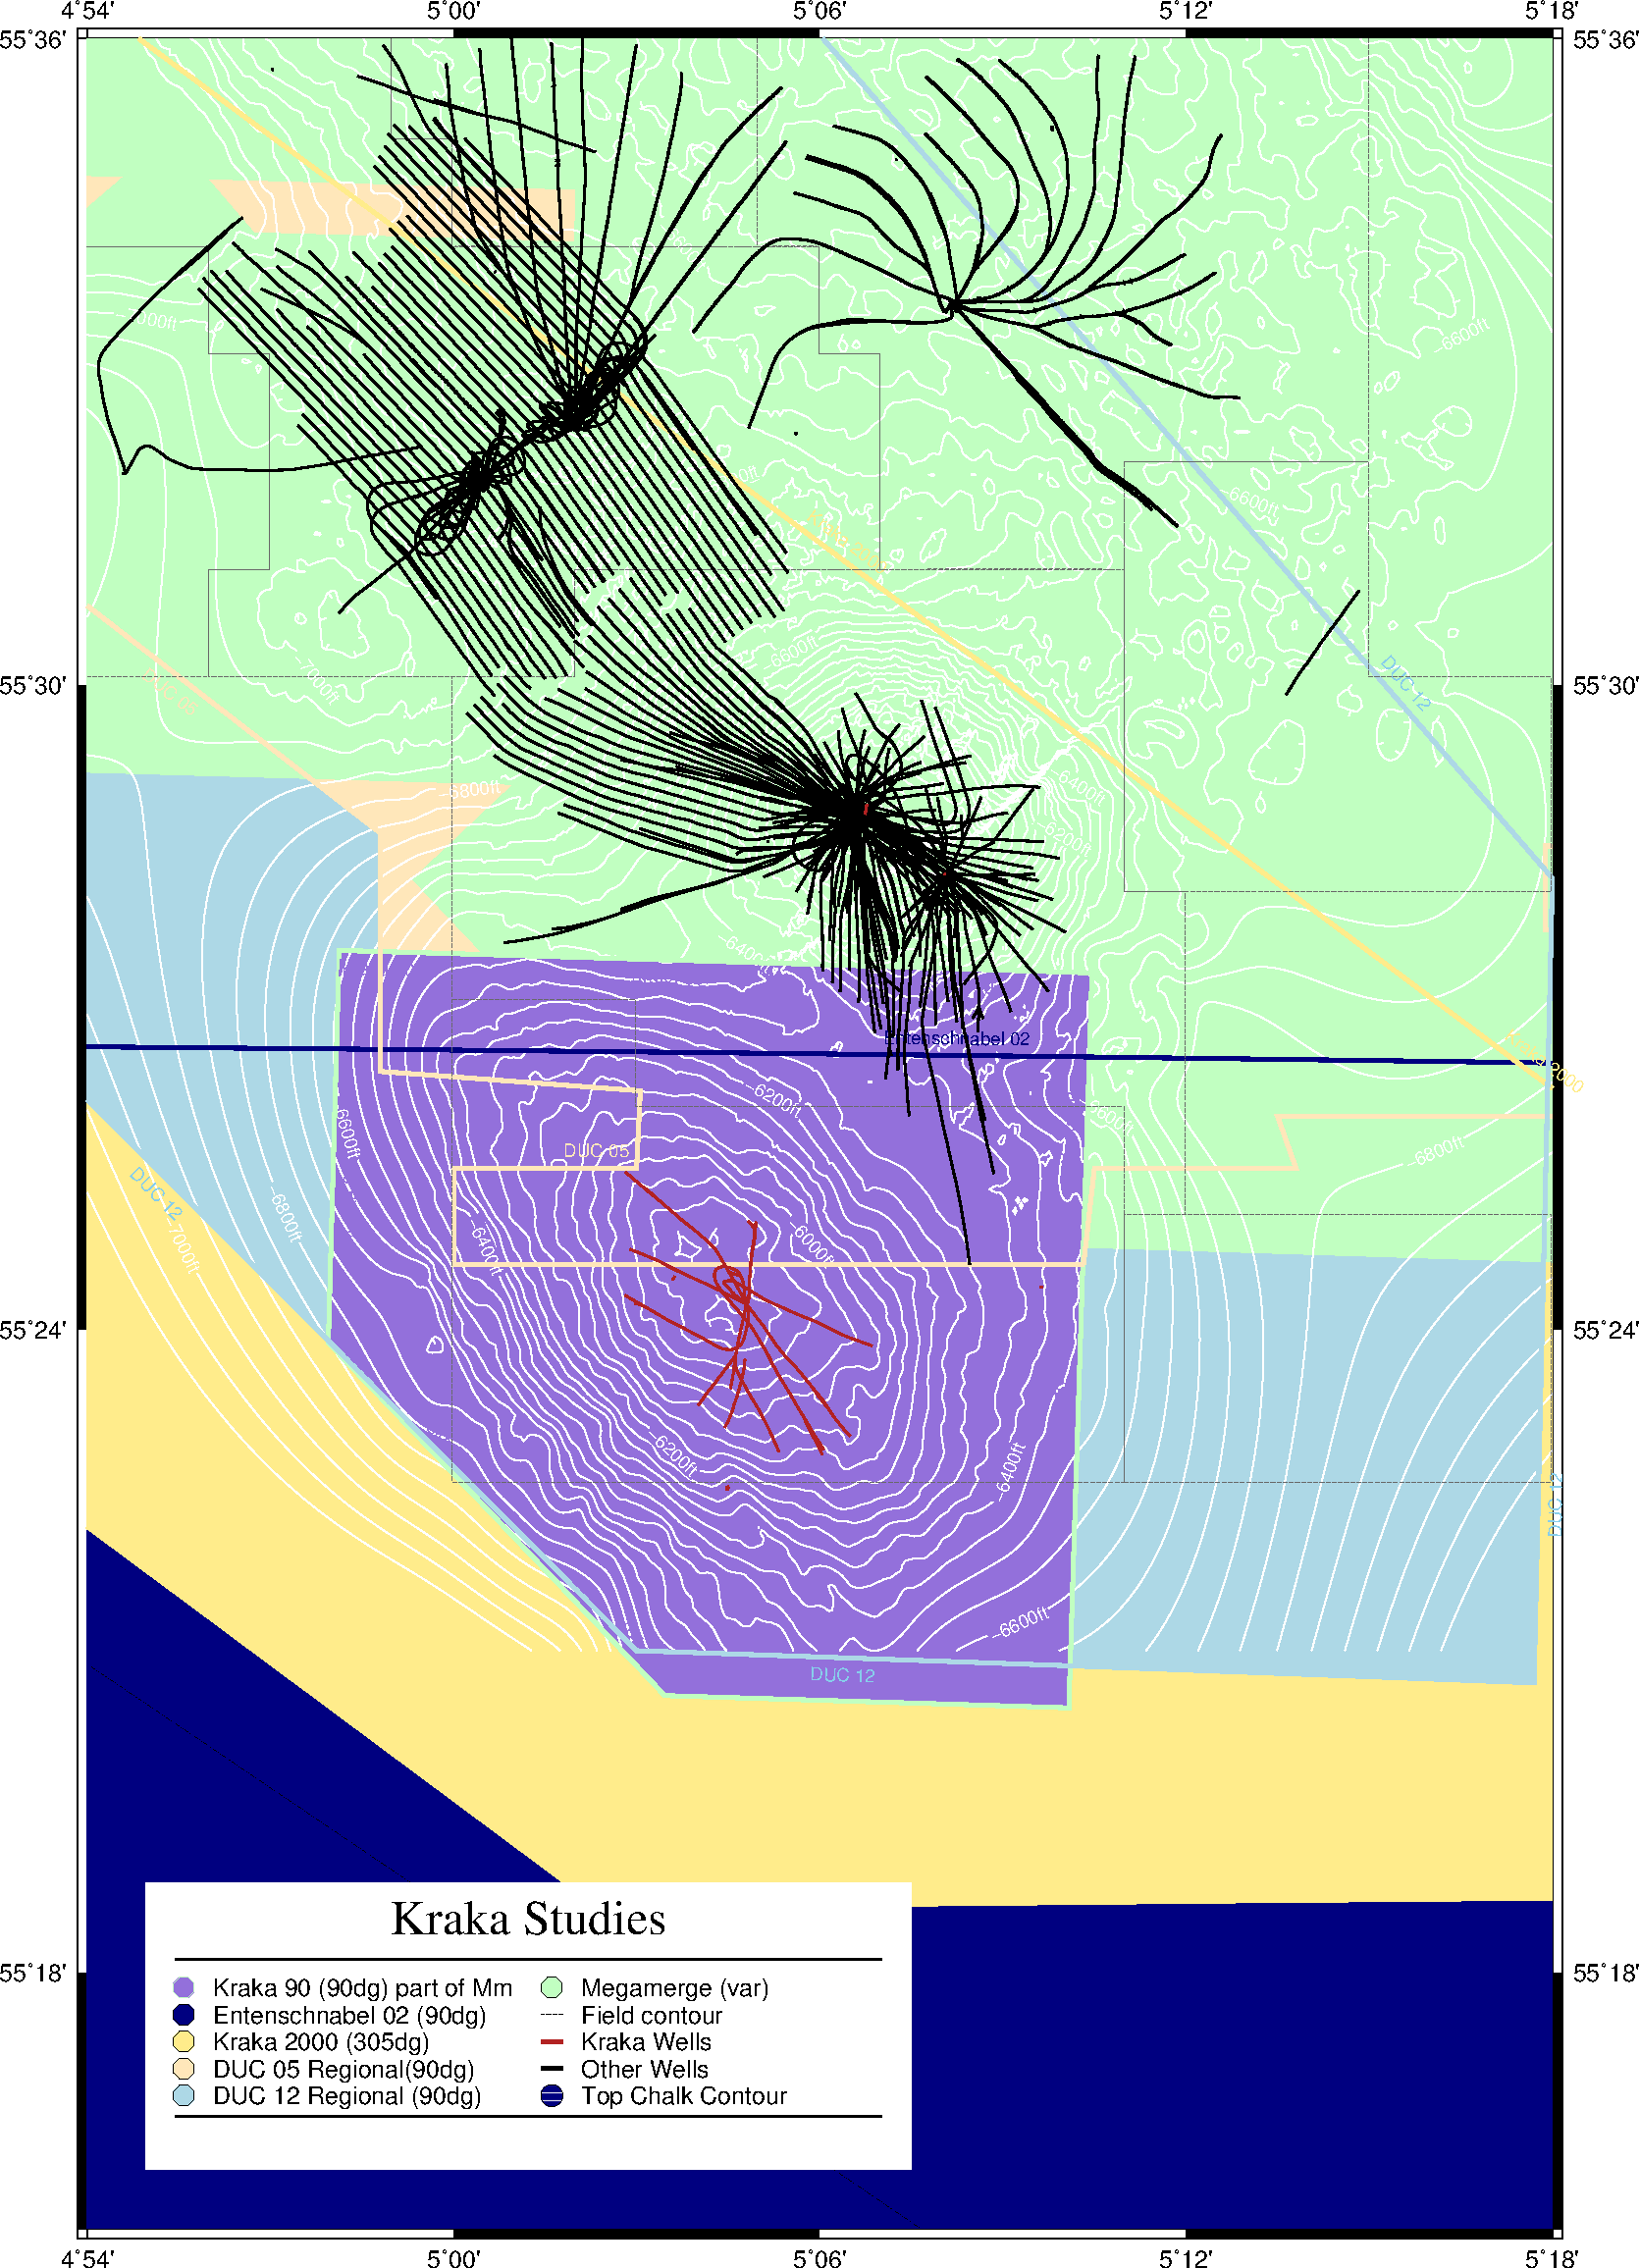
\includepdf[pages={-}]{figures/data/kraka.pdf}

\section*{Dan}
\begin{table}
\centering
\caption{Dan Survey Parameters}
\label{dan-label}
\begin{tabular}{|l|ccccc|}
 \hline
\rowcolor[HTML]{C0C0C0}Survey & \cellcolor[HTML]{C0C0C0}DAN88 & \cellcolor[HTML]{C0C0C0}Kraka00  & \cellcolor[HTML]{C0C0C0}DAN05 & \cellcolor[HTML]{C0C0C0}DUC05 & \cellcolor[HTML]{C0C0C0}DUC12 \\ \hline
Direction [$^o$] & 225 & 305 & 225 & 90 & 90 \\ \hline
Inline Spacing [m] & 12.5 & 12.5 & 12.5 & 6.25 & 6.25 \\ \hline
Crossline Spacing [m] & 12.5 & 12.5 & 12.5 & 25 & 25 \\ \hline
Fold & 50 & & & 60 &  \\ \hline
Undershoot & & No &  & Yes & Yes \\ \hline
\rowcolor[HTML]{C0C0C0} Energy Source & \multicolumn{5}{l|}{\cellcolor[HTML]{C0C0C0}}\\ \hline
Number of Arrays & & 2 & 2 & 2 & 2 \\ \hline
Array Volume [cu.ins.] & 780 & & 3147 & 3147 & 3450 \\ \hline
Source Depth [m] & & & 5 & 5 & 5 \\ \hline
\rowcolor[HTML]{C0C0C0} Streamer Parameters & \multicolumn{5}{l|}{\cellcolor[HTML]{C0C0C0}}\\ \hline
Number of Streamers & 2 & 6 & 8 & 8 & 8 \\ \hline
Separation [m] & 50 & 50 & 100 & 100 \\ \hline 
Length [m] & 2500 & 6000 & 6000 & 4040 \\ \hline
Number of Groups & 200 & 408 & 366 & 478 & 324 \\ \hline
Group Interval [m] & & & 12.5 & 12.5 & 12.5 \\ \hline
Depth [m] & 8 & & 7 & 7 & 7 \\ \hline
Near Offset [m] & & &  & 287 & 102 \\ \hline
\rowcolor[HTML]{C0C0C0} Recording System & \multicolumn{5}{l|}{\cellcolor[HTML]{C0C0C0}}\\ \hline
Low Filter Cut-Off [Hz] & 4 & 4 & 4 & 3 & 3 \\ \hline
Low Filter Flank [dB/Oct] & 18 & 18 &  & 18 & 6 \\ \hline
\end{tabular}
\end{table}
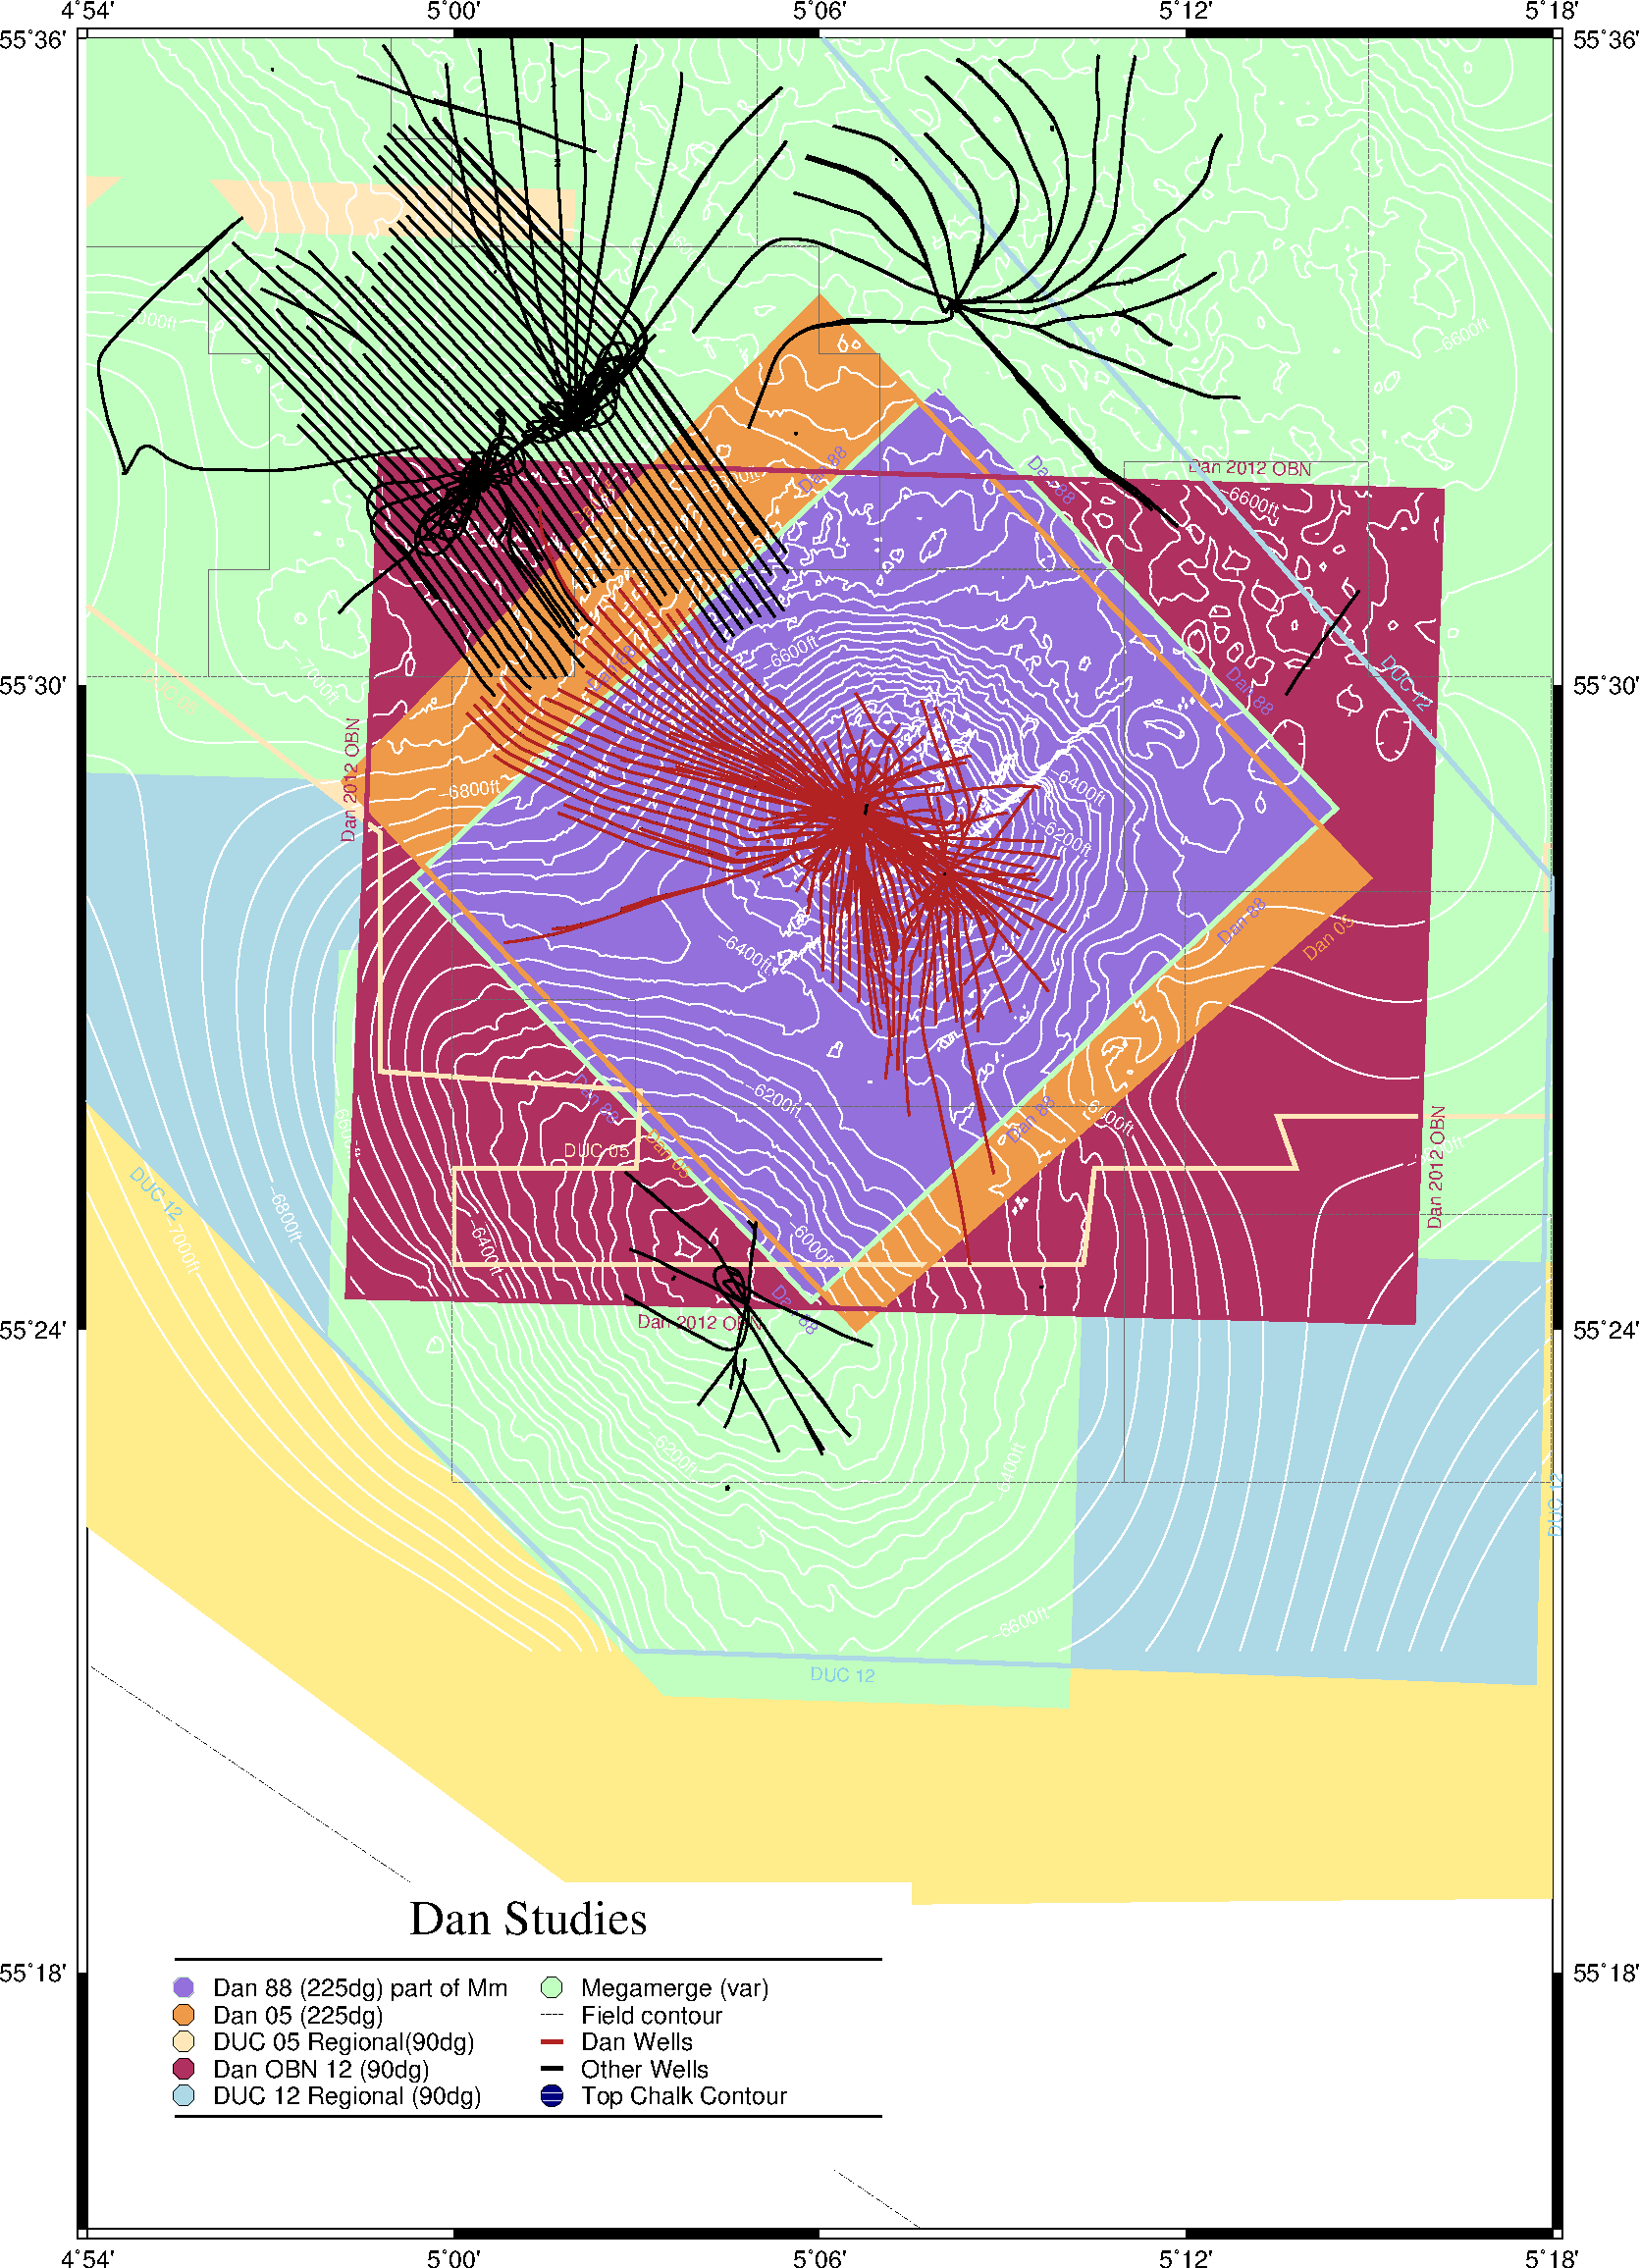
\includepdf[pages={-}]{figures/data/dan.pdf}

\section*{Halfdan}
\begin{table}
\centering
\caption{Halfdan Survey Parameters}
\label{halfdan-label}
\begin{tabular}{|l|ccc|}
\hline
\rowcolor[HTML]{C0C0C0}Survey & \cellcolor[HTML]{C0C0C0}SKJOLD 92 & \cellcolor[HTML]{C0C0C0}DUC05 & \cellcolor[HTML]{C0C0C0}DUC12  \\ \hline
Direction [$^o$] & 90 & 90 & 90  \\ \hline
Inline Spacing [m] & 6.25 & 6.25 & 6.25  \\ \hline
Crossline Spacing [m] & 25 & 25 & 25  \\ \hline
Fold & 30 & 60 &   \\ \hline
Undershoot & Yes & Yes & Yes  \\ \hline
\rowcolor[HTML]{C0C0C0}Energy Source & \multicolumn{3}{l|}{\cellcolor[HTML]{C0C0C0}} \\ \hline
Number of Arrays & 2 & 2 & 2  \\ \hline
Array Volume [cu.ins.] & 1060 & 3147 & 3450  \\ \hline
Source Depth [m] & 5 & 5 & 5  \\ \hline
\rowcolor[HTML]{C0C0C0}Streamer Parameters & \multicolumn{3}{l|}{\cellcolor[HTML]{C0C0C0}} \\ \hline
Number of Streamers & 2 & 8 & 8  \\ \hline
Separation [m] & 100 & 100 & 100  \\ \hline
Length [m] & 3000 & 6000 & 4040  \\ \hline
Number of Groups & 240 & 478 & 324  \\ \hline
Group Interval [m] & 12.5 & 12.5 & 12.5  \\ \hline
Depth [m] & 7 & 7 & 7  \\ \hline
Near Offset [m] & 98 & 287 & 102  \\ \hline
\rowcolor[HTML]{C0C0C0}Recording System & \multicolumn{3}{l|}{\cellcolor[HTML]{C0C0C0}} \\ \hline
Low Filter Cut-Off [Hz] & 8 & 3 & 3  \\ \hline
Low Filter Flank [dB/Oct] & 6 & 18 & 6  \\ \hline
\end{tabular}
\end{table}
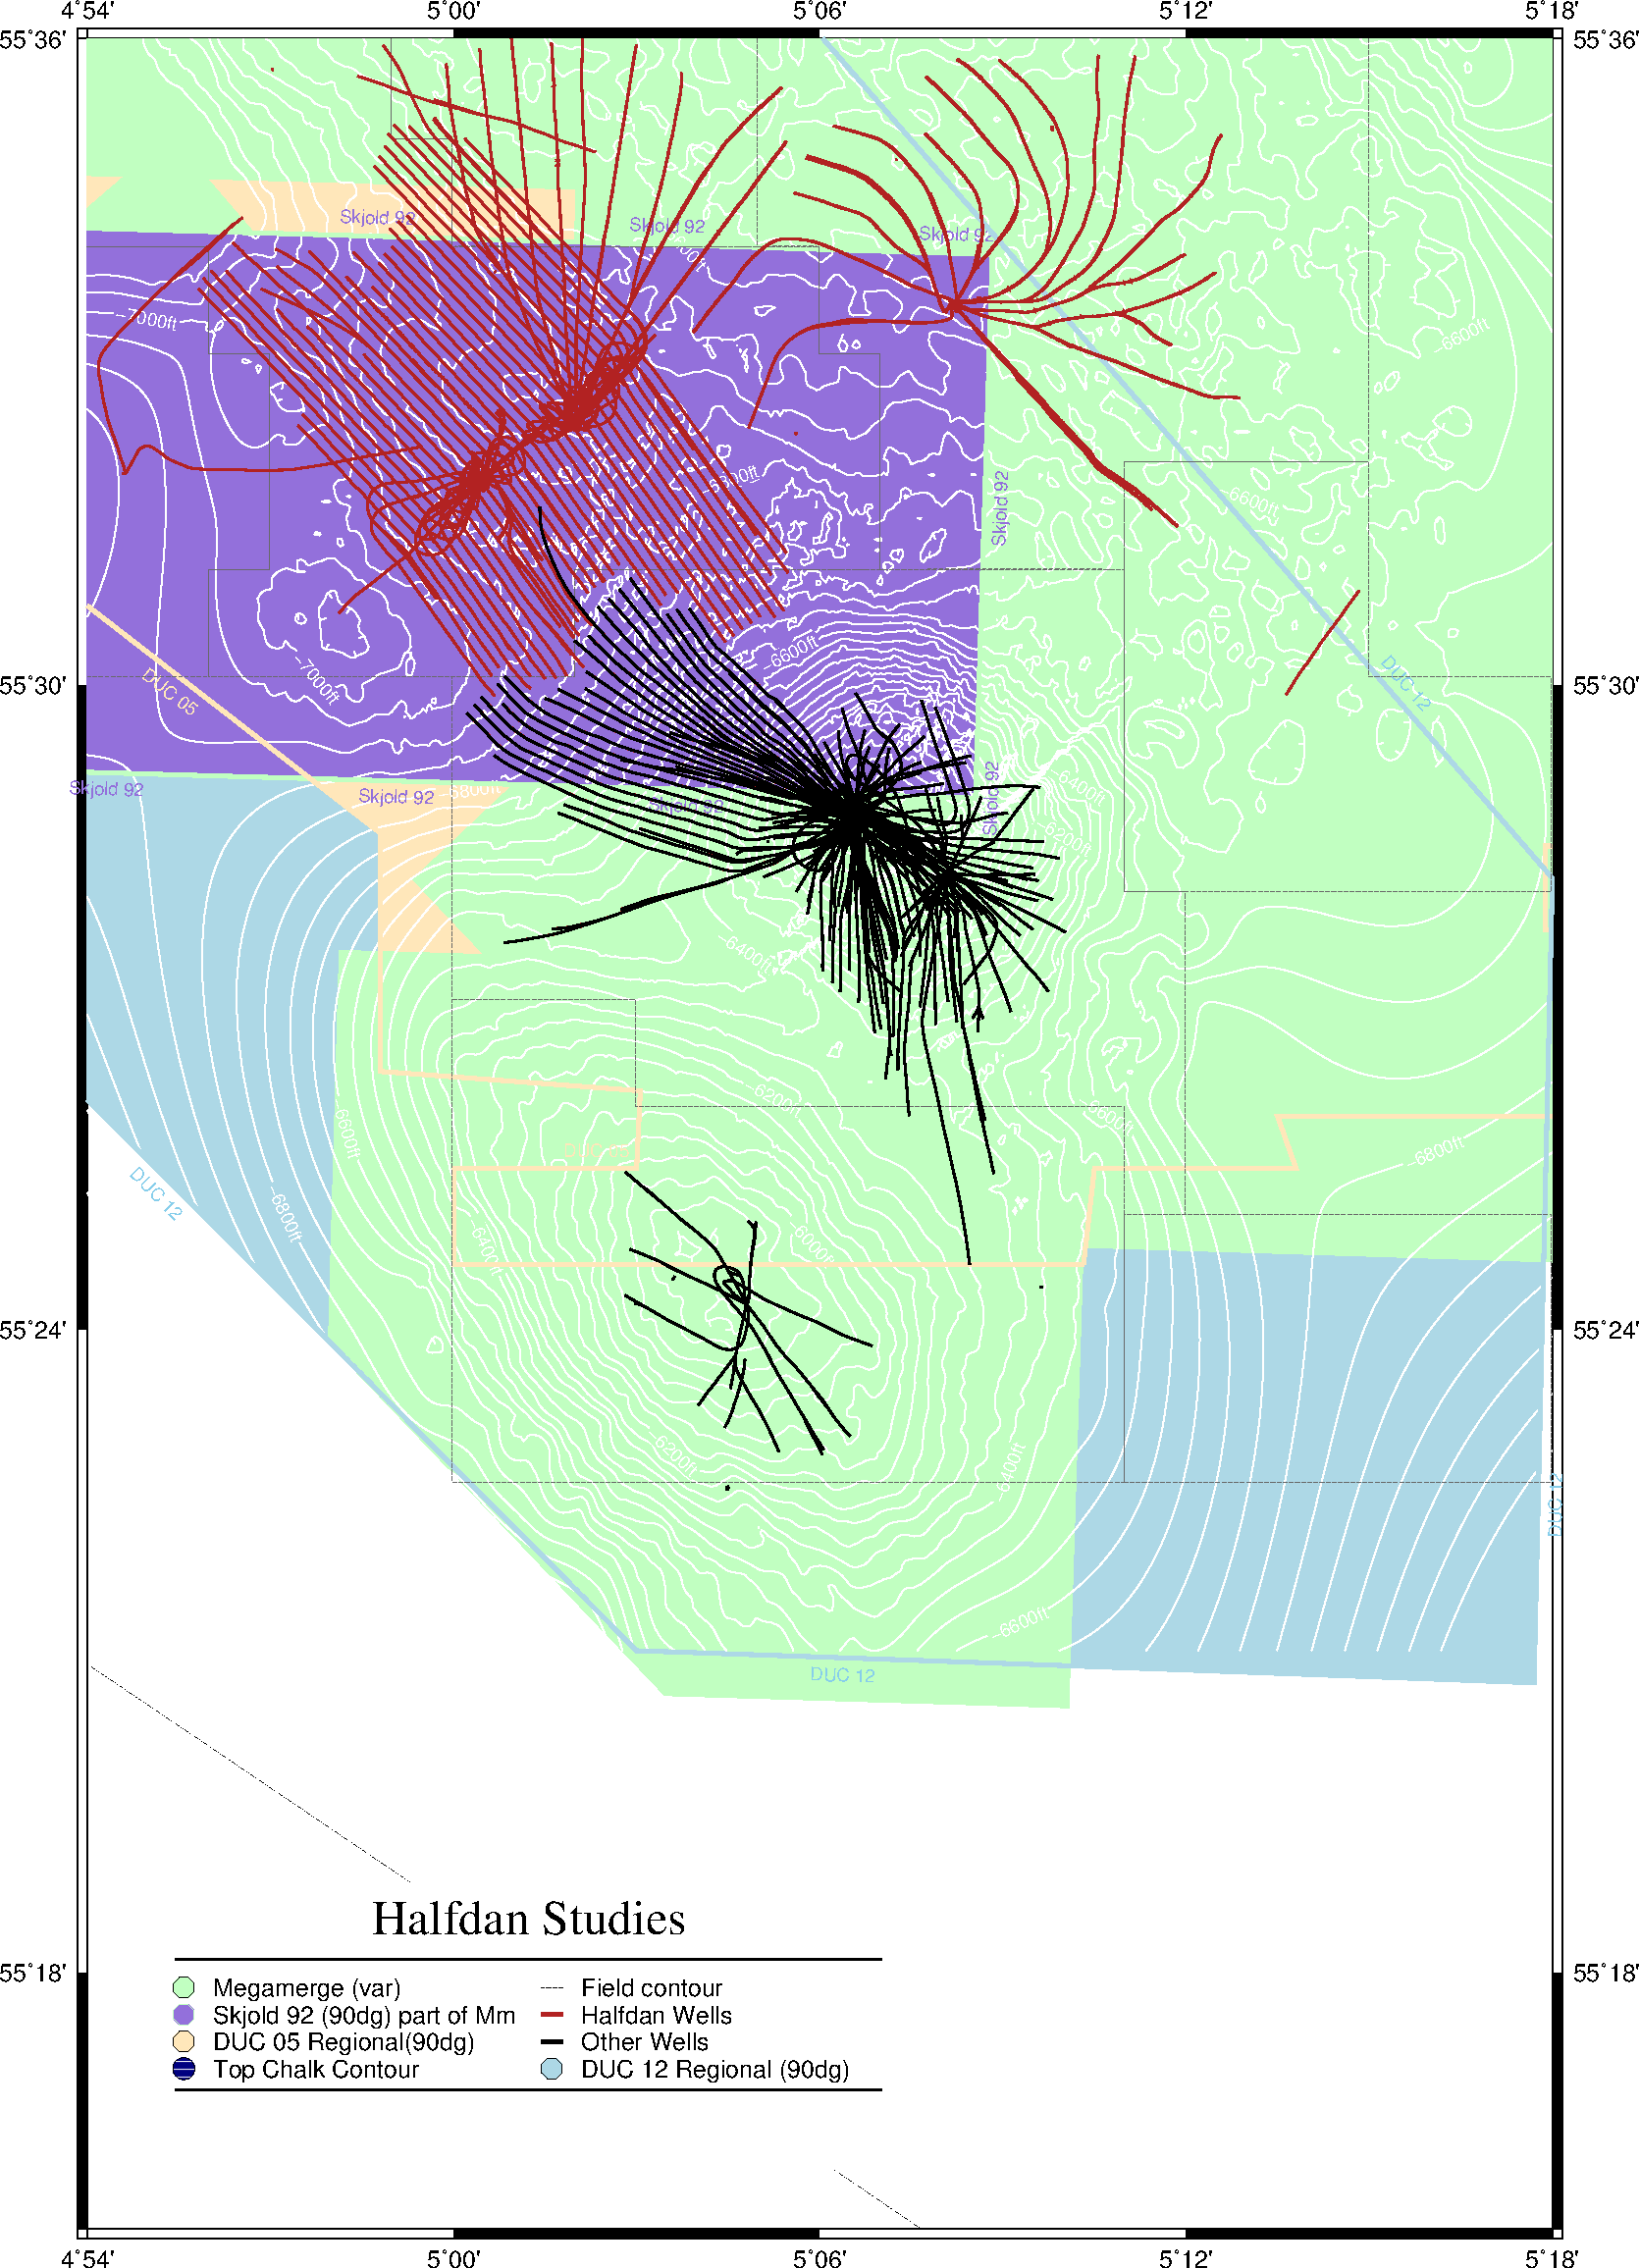
\includepdf[pages={-}]{figures/data/halfdan.pdf}

\begin{landscape}
\section*{Sesimic Surveys}
\begin{table}
    \begin{tabular}{|l|c|c|c|c|c|c|c|c|}
    \hline
    \cellcolor[HTML]{C0C0C0}Survey                    & \cellcolor[HTML]{C0C0C0}DAN88 & \cellcolor[HTML]{C0C0C0}KRAKA90 & \cellcolor[HTML]{C0C0C0}Skjold92 & \cellcolor[HTML]{C0C0C0}KRAKA00 & \cellcolor[HTML]{C0C0C0}ES02 & \cellcolor[HTML]{C0C0C0}DAN05 & \cellcolor[HTML]{C0C0C0}DUC05 & \cellcolor[HTML]{C0C0C0}DUC12 \\ \hline
    Direction [$^o$]       & 225   & 90      & 90       & 305     & 90   & 225   & 90    & 90    \\ \hline
    Inline Spacing [m]        & 12.5  & ~       & 6.25     & 12.5    & 25   & 12.5  & 6.25  & 6.25  \\ \hline
    Crossline Spacing [m]     & 12.5  & ~       & 25       & 12.5    & 12.5 & 12.5  & 25    & 25    \\ \hline
    Fold                      & 50    & ~       & 30       & ~       & ~    & 50    & 60    & ~     \\ \hline
    Undershoot                & ~     & ~       & Yes      & No      & ~    & ~     & Yes   & Yes   \\ \hline
    \multicolumn{9}{|c|}{\cellcolor[HTML]{C0C0C0} Energy Source}    \\ \hline
    Number of Arrays          & ~     & 1       & 2        & 2       & 2    & 2     & 2     & 2     \\\hline
    Array Volume [cu.ins.]    & 780   & 3360    & 1060     & ~       & 3090 & 3147  & 3147  & 3450  \\ \hline
    Source Depth [m]          & ~     & 5       & 5        & ~       & 6    & 5     & 5     & 5     \\ \hline
    \multicolumn{9}{|c|}{\cellcolor[HTML]{C0C0C0}     Streamer Parameters       }    \\ \hline
    Number of Streamers       & 2     & 4       & 2        & 6       & 8    & 8     & 8     & 8     \\ \hline
    Separation [m]            & 50    & 30      & 100      & ~       & ~    & 50    & 100   & 100   \\ \hline
    Length [m]                & 2500  & 288     & 3000     & ~       & 5100 & 6000  & 6000  & 4040  \\ \hline
    Number of Groups          & 200   & 24      & 240      & 408     & 408  & 366   & 478   & 324   \\ \hline
    Group Interval [m]        & ~     & 12.5    & 12.5     & ~       & 12.5 & 12.5  & 12.5  & 12.5  \\ \hline
    Depth [m]                 & 8     & 8       & 7        & ~       & 7    & 7     & 7     & 7     \\ \hline
    Near Offset [m]           & ~     & 80      & 98       & ~       & ~    & ~     & 287   & 102   \\ \hline
    \multicolumn{9}{|c|}{\cellcolor[HTML]{C0C0C0}    Recording System          }    \\ \hline
    Low Filter Cut-Off [Hz]   & 4     & 3       & 8        & 4       & 3    & 4     & 3     & 3     \\ \hline
    Low Filter Flank [dB/Oct] & 18    & 6       & 6        & 18      & 6    & ~     & 18    & 6     \\ \hline
    \multicolumn{9}{|c|}{\cellcolor[HTML]{C0C0C0}Coverage}    \\ \hline
    Kraka                     & ~     & X       & ~        & X       & X    & ~     & \textonehalf     & X    \\ \hline
    Dan                       & X     & ~       & ~        & X       & ~    & X     & X     & X    \\ \hline
    Halfdan                   & ~     & ~       & X        & X       & ~    & ~     & X     & X    \\ \hline
    \end{tabular}
\caption{All Seismic Surveys and fields covered}
\end{table}
\end{landscape}